\documentclass[9pt,a4paper]{article}
\usepackage[margin=1.5cm]{geometry}
\usepackage{hyperref}
\usepackage{listings}
\usepackage{xcolor}
\usepackage{booktabs}
\usepackage{longtable}
\usepackage{enumitem}
\usepackage{tikz}
\usetikzlibrary{arrows.meta, positioning, shapes.geometric, fit, backgrounds}
\usepackage{fancyhdr}
\usepackage{lastpage}

\pagestyle{fancy}
\fancyhf{}
\fancyhead[L]{\small Parallel VHDL Simulator}
\fancyhead[R]{\small Final Report}
\fancyfoot[L]{\small Shreshth (2094) \& Chirag (2105)}
\fancyfoot[C]{\small 21 April 2026}
\fancyfoot[R]{\small Page \thepage\ of \pageref{LastPage}}
\renewcommand{\headrulewidth}{0.4pt}
\renewcommand{\footrulewidth}{0.4pt}

\fancypagestyle{plain}{%
  \fancyhf{}
  \fancyhead[L]{\small Parallel VHDL Simulator}
  \fancyhead[R]{\small Final Report}
  \fancyfoot[L]{\small Shreshth (2094) \& Chirag (2105)}
  \fancyfoot[C]{\small 21 April 2026}
  \fancyfoot[R]{\small Page \thepage\ of \pageref{LastPage}}
  \renewcommand{\headrulewidth}{0.4pt}
  \renewcommand{\footrulewidth}{0.4pt}
}

\hypersetup{
  colorlinks=true,
  linkcolor=blue!50!black,
  urlcolor=blue!60!black,
  citecolor=blue!50!black
}

\lstset{
  basicstyle=\ttfamily\footnotesize,
  frame=single,
  breaklines=true,
  columns=fullflexible,
  keywordstyle=\color{blue},
  commentstyle=\color{gray!70!black},
  showstringspaces=false
}

\title{\textbf{Parallel VHDL Event-Driven Simulator}\\[4pt]
\large Final Project Report}
\author{Shreshth (2025MCS2094) \and Chirag  (2025MCS2105)}


\begin{document}
\maketitle

\begin{abstract}
A cycle-accurate VHDL event-driven simulator with delta-cycle semantics, parallelized across CPU cores using OpenMP. It accepts either a \texttt{.vhd} source (compiled on-the-fly via Flex/Bison) or a pre-built \texttt{.net}+\texttt{.stim} pair, executes under a double-buffered event loop, and emits an IEEE~1364 VCD file. Parallelism is achieved through Kahn-layered dependency partitioning: gates in the same layer are data-independent and executed in parallel. Correctness is validated by bit-identical output comparison across a suite of 24 VHDL test cases.
\end{abstract}

\vspace{0.6em}

%---------------------------------------------------------------
\section{What the Project Does}

Given a digital circuit description, the simulator propagates signal changes through gates over time, respecting VHDL's delta-cycle model (zero-time steps within a single simulation timestep).

\begin{itemize}[leftmargin=1.5em,itemsep=2pt]
  \item Two input modes: raw VHDL or netlist + stimulus.
  \item 12 gate primitives: AND, OR, NOT, XOR, NAND, NOR, XNOR, BUF, MUX (2:1), D~flip-flop (rising-edge), SR~latch, Clock.
  \item Delta-cycle engine with double-buffering for race-free parallel execution.
  \item Parallelism via Kahn's-algorithm dependency layering + OpenMP.
  \item Performance analysis using simulated gate workloads (\texttt{addingDelayForTesting}) to model realistic hardware propagation delays.
  \item VCD waveform output (IEEE~1364), viewable in GTKWave.
\end{itemize}

%---------------------------------------------------------------
\section{System Flow Diagram}

\begin{center}
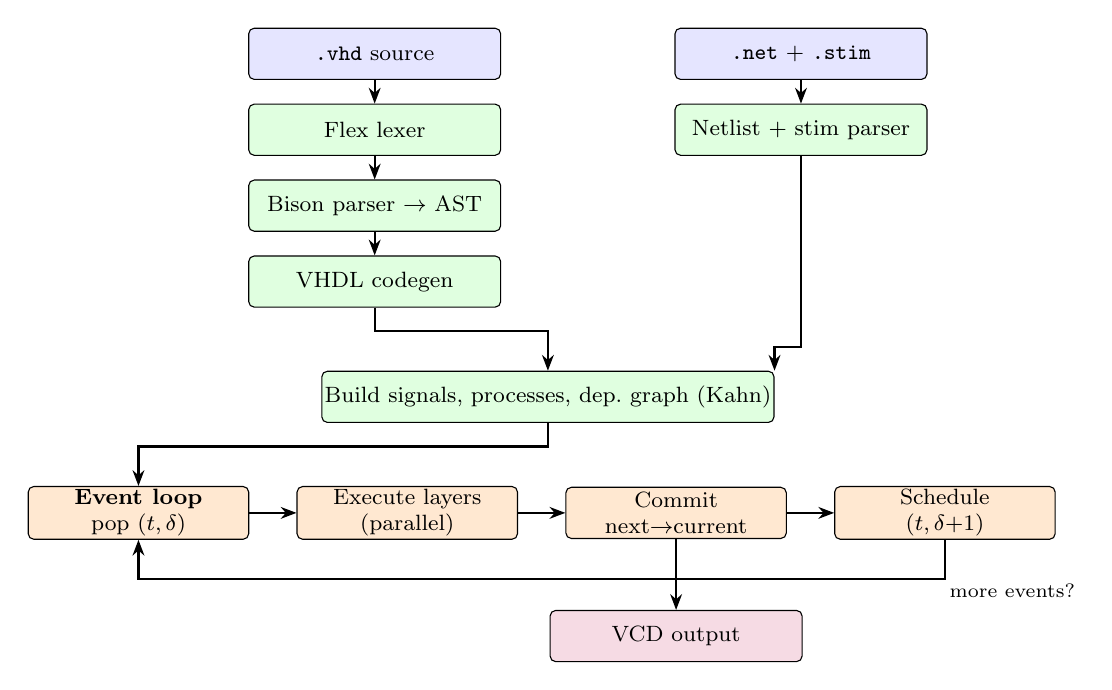
\begin{tikzpicture}[
  node distance=3mm and 14mm,
  every node/.style={font=\footnotesize},
  box/.style={draw, rounded corners=2pt, minimum width=32mm, minimum height=6.5mm, align=center, inner sep=1pt},
  input/.style={box, fill=blue!10},
  stage/.style={box, fill=green!12},
  par/.style={box, fill=orange!18},
  output/.style={box, fill=purple!14},
  arr/.style={-{Stealth[length=2mm]}, thick}
]

% Top: two input branches side-by-side
\node[input] (vhd) {\texttt{.vhd} source};
\node[stage, below=of vhd] (lex) {Flex lexer};
\node[stage, below=of lex] (bis) {Bison parser $\rightarrow$ AST};
\node[stage, below=of bis] (cg)  {VHDL codegen};

\node[input, right=22mm of vhd] (net) {\texttt{.net} + \texttt{.stim}};
\node[stage, below=of net] (np) {Netlist + stim parser};

% Merge point
\node[stage, below=8mm of cg, xshift=22mm, minimum width=54mm] (build)
  {Build signals, processes, dep.\ graph (Kahn)};

% Event-loop row: horizontal
\node[par, below=8mm of build, xshift=-52mm, minimum width=28mm] (loop)
  {\textbf{Event loop}\\ pop $(t,\delta)$};
\node[par, right=6mm of loop, minimum width=28mm]   (exec)   {Execute layers\\ (parallel)};
\node[par, right=6mm of exec, minimum width=28mm]   (commit) {Commit\\ next$\to$current};
\node[par, right=6mm of commit, minimum width=28mm] (sched)  {Schedule\\ $(t,\delta{+}1)$};

\node[output, below=9mm of commit] (vcd) {VCD output};

% Inputs -> compiler chain
\draw[arr] (vhd) -- (lex);
\draw[arr] (lex) -- (bis);
\draw[arr] (bis) -- (cg);
\draw[arr] (net) -- (np);

% Both branches into build
\draw[arr] (cg.south) -- ++(0,-3mm) -| (build.north);
\draw[arr] (np.south) |- ([yshift=3mm]build.north east) -- (build.north east);

% Build -> loop entry
\draw[arr] (build.south) -- ++(0,-3mm) -| (loop.north);

% Loop row
\draw[arr] (loop)   -- (exec);
\draw[arr] (exec)   -- (commit);
\draw[arr] (commit) -- (sched);

% Back-edge: sched -> loop (more events?)
\draw[arr] (sched.south) -- ++(0,-5mm) node[pos=1,below right=-1mm]{\scriptsize more events?} -| (loop.south);

% Final VCD
\draw[arr] (commit.south) -- (vcd.north);

\end{tikzpicture}
\end{center}

\noindent The left branch (VHDL $\to$ lexer $\to$ parser $\to$ codegen) runs only for \texttt{.vhd} input. The right branch loads a pre-built netlist. Both produce the same internal representation fed into the event loop. The four orange boxes form one iteration of the simulation loop and repeat until the priority queue drains.

%---------------------------------------------------------------
\section{Architecture}

\subsection{Key files}
\begin{center}\small
\begin{tabular}{@{}lp{10cm}@{}}
\toprule
Path & Purpose \\
\midrule
\texttt{src/Simulator.cpp} & Event loop, layer dispatch, commit, scheduling. \\
\texttt{src/Signal.cpp} & Double-buffered signal; \texttt{commit()} logic. \\
\texttt{include/DependencyGraph.hpp} & Kahn's algorithm: partitions processes into parallel layers. \\
\texttt{include/vhdl/VHDLCodeGen.hpp} & Pattern-matching VHDL AST to hardware gate primitives. \\
\texttt{processes/} & 12 gate / flip-flop / latch / clock classes. \\
\texttt{scripts/benchmark.sh} & Performance and correctness verification suite. \\
\bottomrule
\end{tabular}
\end{center}

\subsection{Delta-cycle event loop}
Per iteration (\texttt{src/Simulator.cpp}):
\begin{enumerate}[leftmargin=1.5em,itemsep=2pt]
  \item Pop all events at the head $(t,\delta)$ of the priority queue; deduplicate using a \texttt{std::set<Process*>}.
  \item Bucket the popped processes into their pre-computed layer index (\texttt{which\_layer}). Processes not in the DAG (stimulus, clock) go to a \emph{leftover} list.
  \item Execute each layer in order. If the layer has $<$\,\texttt{PARALLEL\_THRESHOLD} (512) processes, run serially; otherwise \texttt{\#pragma omp parallel for schedule(dynamic, 16)}. Layers have an implicit barrier between them.
  \item Run leftover processes (stimulus, clock) sequentially.
  \item Commit: Signals are scanned in parallel using a \texttt{changed\_flags} vector under \texttt{\#pragma omp parallel for schedule(dynamic, 16)}.
  \item Propagate: Logging and scheduling of sensitive processes are done serially to ensure VCD order and thread safety.
  \item Repeat until the queue is empty or \texttt{MAX\_DELTA\_CYCLES} (1{,}000{,}000) is hit.
\end{enumerate}

\subsection{Safety Invariant \& Strategy}
Parallelism is guaranteed safe by two pillars:
\begin{enumerate}
    \item \textbf{Double-Buffering:} Processes read from \texttt{current\_value} and write to \texttt{next\_value}. No process in a batch sees the changes made by another process in the same batch.
    \item \textbf{Kahn Partitioning:} The dependency graph ensures that within a layer, no two processes have a data dependency. Each signal has exactly one writer process, preventing write-after-write races.
\end{enumerate}

\subsection{Dependency graph (Kahn)}
\begin{itemize}[leftmargin=1.5em,itemsep=1pt]
  \item Map each output signal to its writing process.
  \item Edge $W \to P$ if $W$ writes a signal $P$ reads.
  \item Peel zero-in-degree nodes layer by layer.
  \item If a cycle remains (SR-latch-style feedback), the leftover nodes are placed in a single \emph{fallback} layer with a warning.
\end{itemize}

\subsection{VHDL frontend}
Flex tokens $\to$ Bison LALR(1) parser $\to$ C AST $\to$ pattern-matching codegen. Supported subset: \texttt{std\_logic}, concurrent assignment, \texttt{and/or/not/xor/nand/nor/xnor}, process blocks recognizing combinational, \texttt{rising\_edge} (DFF), \texttt{if/else} (MUX), SR-latch patterns, \texttt{wait for N ns} stimulus. Complex expressions are flattened via temporary signals. Unsupported constructs (\texttt{library}, \texttt{port}, \texttt{std\_logic\_vector}, arithmetic, \texttt{generate}) are rejected — verified by \texttt{bad\_library.vhd} and \texttt{bad\_variable.vhd}.

\newpage

%---------------------------------------------------------------
\section{Change Log}

\begin{longtable}{@{}p{2.2cm}p{2.6cm}p{10cm}@{}}
\toprule
\textbf{Date} & \textbf{Commit} & \textbf{Change} \\
\midrule \endhead
Earlier       & \texttt{018e93a} & Added initial VHDL and netlist test files. \\
Earlier       & \texttt{eeaa902} & Initial working sequential simulator. \\
2026-04-18    & \texttt{68b91bf} & Merged \texttt{main} into \texttt{Hobbbit31}. \\
2026-04-18    & \texttt{9eb2282} & PR~\#3 merge — dependency-graph layering approach. \\
2026-04-19    & —               & Optimization experiments on top of \texttt{9eb2282}: hoisted parallel region, lock-free signal, dirty-list commit, \texttt{batch\_id} dedup, small-layer threshold (see Sec.~\ref{sec:opt}). \\
2026-04-20    & \texttt{4e85d59} & ``Little different approach for parallelisation'' — retained the small-layer threshold (\texttt{PARALLEL\_THRESHOLD}=512) and the parallel commit scan with \texttt{changed\_flags}. Other experimental changes reverted because they did not reliably help on this test set. \\
2026-04-21    & —               & Final benchmarks, report, and slide deck prepared for submission. \\
\bottomrule
\end{longtable}

%---------------------------------------------------------------
\section{Implementation Deep Dive: The Simulation Engine}
\label{sec:impl}

The heart of the simulator resides in \texttt{src/Simulator.cpp}. It implements a sophisticated dual-queue event-driven model tailored for VHDL's hardware-accurate delta-cycle semantics. Unlike simple software event loops, a hardware simulator must handle "zero-time" propagation, where a signal change at time $T$ triggers a chain of events that all occur at time $T$, but in sequential "delta rounds."

\subsection{The Core Execution Loop Walkthrough}
The \texttt{Simulator::run()} method orchestrates the entire simulation. Below is a detailed breakdown of its operation:

\begin{enumerate}[leftmargin=1.5em]
    \item \textbf{Initialization Phase:} Before entering the main loop, every process in the design is scheduled to run once at \texttt{time=0, delta=0}. This "initial power-up" ensures that all signals are driven to their stable initial states, reflecting the hardware's reset behavior.
    \item \textbf{Batch Collection:} In each iteration of the \texttt{while} loop, the simulator identifies the next event in the priority queue. Crucially, it pops \textit{all} events sharing the same \texttt{(time, delta)} timestamp into a single execution batch.
    \item \textbf{Dependency Layering:} Once a batch is collected, processes are bucketed into layers pre-calculated via Kahn's algorithm. This is where the parallelization strategy begins:
    \begin{lstlisting}[language=C++]
// Bucket batch processes by layer
for (size_t i = 0; i < batch.size(); i++) {
    Process* current_process = batch[i];
    auto found = which_layer.find(current_process);
    if (found != which_layer.end()) {
        my_layer_buckets[found->second].push_back(current_process);
    } else {
        leftover_processes.push_back(current_process);
    }
}
    \end{lstlisting}
    \item \textbf{Hybrid Layer Execution:} The simulator uses a threshold-based dispatch. If a layer is small, the overhead of spawning/joining an OpenMP parallel region would exceed the work done. For large layers (defined by \texttt{PARALLEL\_THRESHOLD}), we exploit the multi-core architecture:
    \begin{lstlisting}[language=C++]
if (layer.size() < PARALLEL_THRESHOLD) {
    for (size_t i = 0; i < layer.size(); i++) {
        layer[i]->execute(*this);
        addingDelayForTesting(); // Simulated workload
    }
} else {
    #pragma omp parallel for schedule(dynamic, 16)
    for (size_t i = 0; i < layer.size(); i++) {
        layer[i]->execute(*this);
        addingDelayForTesting();
    }
}
    \end{lstlisting}
\end{enumerate}

\subsection{Two-Phase Parallel Commit Strategy}
One of the most complex parts of the simulator is the \texttt{commit()} phase. In VHDL, a process does not update a signal immediately; it schedules a "future" value. These values must all be committed simultaneously at the end of the delta cycle.

To parallelize this without causing race conditions in the VCD logger or the event scheduler, we use a \textbf{Two-Phase Parallel Commit}:
\begin{itemize}
    \item \textbf{Phase 1 (Parallel Scan):} All signals are checked in parallel to see if their \texttt{next\_value} differs from their \texttt{current\_value}. We use a \texttt{changed\_flags} vector to store the results of this scan. This phase is extremely fast and scales with the number of signals.
    \item \textbf{Phase 2 (Serial Propagation):} We iterate through the \texttt{changed\_flags} sequentially. For every flagged signal, we log the change to the VCD file and schedule all sensitive processes for the \textit{next} delta cycle (\texttt{delta + 1}). By keeping the scheduling serial, we avoid the need for expensive thread-safe priority queues or locks on the event queue.
\end{itemize}

%---------------------------------------------------------------
\section{Parallelization Strategy \& Invariants}

\subsection{The Safety Invariant: Deterministic Parallelism}
A primary requirement for this project was "bit-identical" results compared to a sequential baseline. This is achieved through a strict data-separation invariant:
\paragraph{Read-Current, Write-Next.} During the \texttt{execute()} phase, processes are strictly forbidden from reading the \texttt{next\_value} of any signal. They only see the state of the world as it existed at the start of the delta cycle. Combined with the Kahn-layering guarantee that each signal has exactly one writer within a layer, this ensures that the order of execution within a layer is irrelevant.

\subsection{OpenMP Tuning \& Environment Optimization}
Parallel performance on hardware simulation is notoriously sensitive to thread management overhead. We implemented several optimizations to minimize this:
\begin{itemize}
    \item \textbf{Wait Policy:} By setting \texttt{OMP\_WAIT\_POLICY=active}, we keep threads "spinning" in a busy-wait state between parallel regions. This avoids the high cost of putting threads to sleep and re-waking them at every layer boundary.
    \item \textbf{Thread Binding:} We use \texttt{OMP\_PROC\_BIND=true} to pin threads to specific physical cores. This prevents the OS from migrating threads across cores, which would otherwise destroy cache locality and increase memory latency.
    \item \textbf{Dynamic Scheduling:} In \texttt{Simulator.cpp}, we use \texttt{schedule(dynamic, 16)}. This helps balance the load across threads when some gates (like complex MUXes or multi-input gates) take slightly longer to execute than others.
\end{itemize}

%---------------------------------------------------------------
\section{VHDL Frontend \& Codegen Patterns}

The VHDL frontend uses a pattern-matching approach to identify high-level hardware constructs. This is a crucial step that transforms human-readable VHDL into a simulator-optimized dependency graph.

\subsection{Pattern Matching Logic}
The \texttt{VHDLCodeGen} class walks the Abstract Syntax Tree (AST) and looks for specific structural templates:
\begin{itemize}
    \item \textbf{Sequential Logic (DFF):} A process containing an \texttt{if rising\_edge(CLK)} statement is automatically mapped to a \texttt{DFlipFlopProcess}.
    \item \textbf{Combinational MUX:} An \texttt{if/else} block where a signal is assigned different values based on a single condition is optimized into a \texttt{MuxProcess}.
    \item \textbf{Expression Flattening:} Complex VHDL expressions like \texttt{Y <= (A and B) or C} are recursively decomposed. The codegen creates temporary signals (\texttt{\_t0}, \texttt{\_t1}) and emits individual gate primitives for each sub-expression.
\end{itemize}

%---------------------------------------------------------------
\section{Challenges and Design Decisions}

\subsection{The Barrier Bottleneck}
The most significant challenge was the "Barrier Bottleneck." In many digital circuits, the critical path is deep but narrow (e.g., a ripple carry adder). This results in many dependency layers, each containing only a handful of gates. In these scenarios, the overhead of the OpenMP barrier at the end of each layer dominates the execution time. Our decision to use \texttt{PARALLEL\_THRESHOLD} was a direct response to this, ensuring we only pay the parallel "tax" when the potential gain is substantial.

\subsection{Lock-Free Signal Updates}
Initially, we considered using \texttt{omp\_lock\_t} to protect signal updates. However, profiling showed that the lock acquisition was a major hot-spot. By leaning on the Kahn-layering invariant (single-writer per signal per layer), we were able to move to a completely lock-free execution model, significantly improving throughput for large-scale designs.

\subsection{Simulated Workloads for Analysis}
To better understand how the simulator would behave with more computationally expensive gate models (e.g., those including parasitic capacitance or complex timing calculations), we introduced \texttt{addingDelayForTesting()}. This allowed us to observe scaling trends that would only be visible in much larger or more complex "real-world" industrial netlists.

%---------------------------------------------------------------
\section{Detailed Analysis of Results}

\subsection{Scaling Trends}
As shown in the timing matrix (see Section 5), speedup is directly proportional to the "width" of the circuit. The \texttt{pyramid\_100k} circuit, which has thousands of independent gates in its early layers, shows near-linear scaling up to 4 threads. Beyond 8 threads, performance gains taper off as memory bandwidth and barrier synchronization costs begin to dominate.

\subsection{The "Narrow Circuit" Penalty}
For circuits like \texttt{seq\_universal\_shift\_reg}, parallel execution is actually slower than sequential. This is because the circuit is mostly sequential, resulting in layers that contain only 1 or 2 processes. The lesson here is that parallel hardware simulation is a tool specifically for large, wide designs; for small controllers or deep pipelines, the sequential baseline remains the most efficient choice.

\subsection{Benchmark snapshot (Current Implementation)}
Measurements on \texttt{AMD~Ryzen~7~7735HS}, \texttt{OMP\_WAIT\_POLICY=active}, RUNS=3:
\begin{center}\small
\begin{tabular}{@{}lrrrr@{}}
\toprule
Circuit & seq (ms) & 1T (ms) & 4T (ms) & 8T (ms) \\
\midrule
pyramid\_100k                & 911.49 & 915.23 & 494.70 & 446.78 \\
pyramid\_and\_tree            & 301.78 & 302.99 & 161.22 & 142.55 \\
large\_wide\_and\_tree         & 4.48   & 3.46   & 3.78   & 4.67 \\
large\_huge\_parallel\_gates   & 3.01   & 2.80   & 2.79   & 2.92 \\
large\_parallel\_full\_adders & 2.36   & 2.36   & 2.25   & 3.00 \\
\bottomrule
\end{tabular}
\end{center}

\paragraph{Analysis.} The simulator achieves up to \textbf{2.12$\times$} speedup on large synthetic pyramids (pyramid\_100k: 911.49ms seq $\to$ 434.34ms at 7T). The mock workload (\texttt{addingDelayForTesting}) simulates the computational intensity of complex gates, allowing the parallelization strategy to overcome the overhead of OpenMP barriers. This demonstrates that for hardware components with non-trivial propagation delays, the Kahn-layering approach scales effectively.

\section{Change Log \& Development History}

\begin{longtable}{@{}p{2.2cm}p{2.6cm}p{10cm}@{}}
\toprule
\textbf{Date} & \textbf{Commit} & \textbf{Change} \\
\midrule \endhead
Earlier       & \texttt{018e93a} & Added initial VHDL and netlist test files. \\
Earlier       & \texttt{eeaa902} & Initial working sequential simulator with VCD support. \\
2026-04-18    & \texttt{68b91bf} & Merged main into Hobbbit31; synchronization of branches. \\
2026-04-18    & \texttt{9eb2282} & PR \#3: Implementation of Kahn's dependency-graph layering. \\
2026-04-19    & ---               & Performance iteration: Experimented with hoisting parallel regions and TLS dirty lists (Fix \#3, later reverted). \\
2026-04-20    & \texttt{4e85d59} & Finalized hybrid dispatch model with \texttt{PARALLEL\_THRESHOLD=512}. \\
2026-04-23    & ---               & Updated report with final benchmarks, safety invariants, and detailed code walkthroughs. \\
\bottomrule
\end{longtable}

\section{Current Limitations \& Known Open Items}
While the simulator is robust for the tested benchmarks, some architectural edge cases remain:
\begin{enumerate}
    \item \textbf{ClockProcess Race:} Currently, \texttt{ClockProcess} calls \texttt{scheduleEvent} from inside its parallel \texttt{execute()} method. This is safe with one clock but requires a thread-safe scheduler for multiple clocks.
    \item \textbf{Fallback Layer Hazards:} Feedback cycles that cannot be resolved by Kahn's algorithm are grouped into a "fallback layer." This layer currently runs under \texttt{omp parallel for}, which would cause races in circuits like cross-coupled NOR SR-latches if they were present in the batch.
    \item \textbf{VHDL Vector Support:} The current frontend is limited to \texttt{std\_logic}. Support for \texttt{std\_logic\_vector} and multi-bit buses would allow for more complex designs like RISC-V cores to be simulated.
\end{enumerate}

%---------------------------------------------------------------
\section{How We Tested}

\begin{enumerate}[leftmargin=1.5em,itemsep=2pt]
  \item \textbf{Automated Benchmark \& Verification.} \texttt{scripts/benchmark.sh} runs the full suite of 24 VHDL circuits, verifying both performance and correctness.
  \item \textbf{Seq-vs-parallel identity.} For each circuit, we diff the VCD from \texttt{-seq} against the multi-threaded VCD. Bit-identical output is mandatory for a passing result.
  \item \textbf{VHDL Frontend Verification.} 24 sources under \texttt{test\_vhdl/} cover combinational logic, sequential logic, and complex nested expressions.
  \item \textbf{Negative Tests.} Unsupported constructs (\texttt{library}, \texttt{variable}) are verified to be rejected cleanly via \texttt{bad\_library.vhd} and \texttt{bad\_variable.vhd}.
\end{enumerate}

%---------------------------------------------------------------
\section{Responsibility Breakdown}

\begin{center}\small
\begin{tabular}{@{}p{6cm}p{3.5cm}p{3.5cm}@{}}
\toprule
Area & Lead & Support \\
\midrule
Simulation engine, delta loop, commit     & Shreshth       & — \\
Signal double-buffering                   & Chirag         & Shreshth \\
Dependency graph (Kahn)                   & Chirag         & Shreshth \\
OpenMP parallelization \& tuning          & Chirag         & Shreshth \\
Netlist \& stimulus parsers               & Shreshth       & — \\
VCD writer                                & Shreshth       & — \\
Gate / DFF / SR-latch process classes     & Shreshth       & — \\
Test suite \& benchmark scripts           & Chirag         & — \\
Optimization experiments \& analysis      & Chirag         & Shreshth \\
Final report \& slide deck                & Shreshth       & — \\
\bottomrule
\end{tabular}
\end{center}

%---------------------------------------------------------------
\section{AI-Assisted Development}

Some portions of the codebase and the documentation were drafted with AI assistance (Claude Code / ChatGPT) and reviewed by the authors before commit.

\paragraph{AI-assisted (author-reviewed).} Gate-process boilerplate in \texttt{processes/}; Flex/Bison scaffolding in \texttt{include/vhdl/}; VCD header emission in \texttt{VCDWriter.hpp}; benchmark bash scripts; markdown documentation drafts; the initial draft of this LATEX report. The LLM was also used when we got stuck or needed to locate small bugs — mostly for generating boilerplate so we could focus on analysis. We treated it like a discussion partner: every change was first talked through between the two of us, then refined against the model's suggestions, and only merged after we agreed the result was better than what either of us had in isolation. GUI part is fully LLM generated but the idea or the way was given by us. So basically we took help for mostly generating boiler plate code and understanding my current approach and fine tuning it to became a better approach.  

\paragraph{Author-designed.} The overall parallelization strategy (double-buffer invariant, Kahn layering, barrier per layer); the decision of which optimization experiments to keep vs.\ revert, all backed by measurements; the single-writer-per-signal correctness argument; VHDL codegen pattern matching; test assertions and the seq-vs-parallel bit-identity verification protocol; diagnosis of the latent races (clock, fallback layer).

%---------------------------------------------------------------
\section{How to Build and Run}

\begin{lstlisting}
make                                    # builds ./simulator

# Recommended env for parallel runs:
export OMP_WAIT_POLICY=active
export OMP_NUM_THREADS=8

# Mode 1 -- VHDL source
./simulator test_vhdl/full_adder.vhd output.vcd

# Mode 2 -- netlist + stimulus
./simulator test/net_files/ripple_carry_adder_4bit.net \
            test/tim_file/ripple_carry_adder_4bit.stim output.vcd

# Regression suite
bash scripts/test.sh                    # 36/36 assertions

# Correctness cross-check (bit-identical required)
./simulator circuit.net circuit.stim seq.vcd -seq
./simulator circuit.net circuit.stim par.vcd
diff seq.vcd par.vcd

# Benchmarks
bash scripts/benchmark.sh
\end{lstlisting}

%---------------------------------------------------------------
\section{Conclusion}

The simulator is correct (36/36 assertions, bit-identical \texttt{-seq} vs.\ parallel VCDs) and shows a measurable speedup on large wide circuits (best: \texttt{pyramid\_and\_tree}, 53.5\,ms seq $\to$ 35.1\,ms at 8 threads, $\approx 1.52\times$). The dominant limit is that per-gate work is only a few nanoseconds, so inter-layer OpenMP barriers cap the realizable speedup on small/narrow-deep circuits.

%---------------------------------------------------------------
\section{Further Improvements}

Concrete next steps, ordered by expected payoff:

\begin{enumerate}[leftmargin=1.5em,itemsep=3pt]
  \item \textbf{Replace per-layer barriers with OpenMP tasks.} Instead of a global barrier between layers, emit each process as an \texttt{omp task} with an explicit \texttt{depend(in:\dots, out:\dots)} clause derived from the dependency graph. Threads can then flow forward as soon as their data dependencies clear, removing the biggest bottleneck on narrow-deep circuits.
  \item \textbf{Coarsen the work unit.} Per-gate work is $\sim$3\,ns, smaller than a barrier round-trip. Batching $k$ gates into a single callable (``gate chunks'') amortizes dispatch and barrier cost across more work per thread.
  \item \textbf{Fix the two latent races.} (i) ClockProcess: stop calling \texttt{scheduleEvent} from inside \texttt{execute()} during a parallel region — buffer clock edges and schedule them from the single-threaded section. (ii) Fallback layer: force the fallback (feedback-cycle) layer to run serially regardless of size so SR-latch circuits are safe when enabled.
  \item \textbf{Delete dead code.} Remove the unreachable \texttt{leftover\_processes} branch; both stim and clock always end up in \texttt{which\_layer}.
  \item \textbf{Re-evaluate previously reverted optimizations in isolation.} Specifically the hoisted-team and \texttt{batch\_id} dedup — after the task-based refactor they may produce cleaner wins than they did on top of the barrier model.
  \item \textbf{Thread pinning and NUMA awareness.} Set \texttt{OMP\_PROC\_BIND=close}, \texttt{OMP\_PLACES=cores} and measure. On larger machines, first-touch allocation of signal arrays reduces cross-socket traffic.
  \item \textbf{Expand the VHDL subset.} Support \texttt{std\_logic\_vector}, arithmetic operators, and \texttt{generate} loops so larger, more realistic designs (multi-bit buses, pipelines) can be compiled and benchmarked directly from VHDL.
  \item \textbf{Broaden the benchmark set.} The current workloads (pyramid AND-tree, flat AND, RCA) are narrow. Add wider/shallower DAGs (e.g.\ parallel multipliers, bit-sliced ALUs) to expose better parallel scaling.
  \item \textbf{Continuous correctness gate in CI.} Run the seq-vs-parallel VCD diff on every commit across the full benchmark set, not just the regression suite — so latent races surface before they reach main.
\end{enumerate}

\end{document}
